% Template file for an a0 landscape poster.
% Written by Graeme, 2001-03 based on Norman's original microlensing
% poster.
%
% See discussion and documentation at
% <http://www.astro.gla.ac.uk/users/norman/docs/posters/> 
%
% $Id: poster-template-landscape.tex,v 1.2 2002/12/03 11:25:46 norman Exp $


% Default mode is landscape, which is what we want, however dvips and
% a0poster do not quite do the right thing, so we end up with text in
% landscape style (wide and short) down a portrait page (narrow and
% long). Printing this onto the a0 printer chops the right hand edge.
% However, 'psnup' can save the day, reorienting the text so that the
% poster prints lengthways down an a0 portrait bounding box.
%
% 'psnup -w85cm -h119cm -f poster_from_dvips.ps poster_in_landscape.ps'

\documentclass[a0]{a0poster}
% You might find the 'draft' option to a0 poster useful if you have
% lots of graphics, because they can take some time to process and
% display. (\documentclass[a0,draft]{a0poster})
\input defs.tex
\pagestyle{empty}
\setcounter{secnumdepth}{0}
\renewcommand{\familydefault}{\sfdefault}
\newcommand{\QED}{~~\rule[-1pt]{8pt}{8pt}}\def\qed{\QED}

\renewcommand{\reals}{{\mbox{\bf R}}}

\usepackage{amsmath}

% The textpos package is necessary to position textblocks at arbitary 
% places on the page.
\usepackage[absolute]{textpos}

\usepackage{fleqn,psfrag,wrapfig}

\usepackage[papersize={38in,28in}]{geometry}

% Graphics to include graphics. Times is nice on posters, but you
% might want to switch it off and go for CMR fonts.
\usepackage{graphics}


% we are running pdflatex, so convert .eps files to .pdf
\usepackage[pdftex]{graphicx}
\usepackage{epstopdf}

% These colours are tried and tested for titles and headers. Don't
% over use color!
\usepackage{color}
\definecolor{Red}{rgb}{0.9,0.0,0.1}

\definecolor{bluegray}{rgb}{0.15,0.20,0.40}
\definecolor{bluegraylight}{rgb}{0.35,0.40,0.60}
\definecolor{gray}{rgb}{0.3,0.3,0.3}
\definecolor{lightgray}{rgb}{0.7,0.7,0.7}
\definecolor{darkblue}{rgb}{0.2,0.2,1.0}
\definecolor{darkgreen}{rgb}{0.0,0.5,0.3}

\renewcommand{\labelitemi}{\textcolor{bluegray}\textbullet}
\renewcommand{\labelitemii}{\textcolor{bluegray}{--}}

\setlength{\labelsep}{0.5em}


% see documentation for a0poster class for the size options here
\let\Textsize\normalsize
%\def\Head#1{\noindent\hbox to \hsize{\hfil{\LARGE\color{bluegray} #1}}\bigskip}
\def\Head#1{\noindent{\LARGE\color{bluegray} #1}\bigskip}
\def\LHead#1{\noindent{\LARGE\color{bluegray} #1}\bigskip}
\def\Subhead#1{\noindent{\large\color{bluegray} #1}\bigskip}
\def\Title#1{\noindent{\VeryHuge\color{Red} #1}}


% Set up the grid
%
% Note that [40mm,40mm] is the margin round the edge of the page --
% it is _not_ the grid size. That is always defined as 
% PAGE_WIDTH/HGRID and PAGE_HEIGHT/VGRID. In this case we use
% 23 x 12. This gives us three columns of width 7 boxes, with a gap of
% width 1 in between them. 12 vertical boxes is a good number to work
% with.
%
% Note however that texblocks can be positioned fractionally as well,
% so really any convenient grid size can be used.
%
\TPGrid[40mm,40mm]{23}{12}      % 3 cols of width 7, plus 2 gaps width 1

\parindent=0pt
\parskip=0.2\baselineskip

\begin{document}

% Understanding textblocks is the key to being able to do a poster in
% LaTeX. In
%
%    \begin{textblock}{wid}(x,y)
%    ...
%    \end{textblock}
%
% the first argument gives the block width in units of the grid
% cells specified above in \TPGrid; the second gives the (x,y)
% position on the grid, with the y axis pointing down.

% You will have to do a lot of previewing to get everything in the 
% right place.

% This gives good title positioning for a portrait poster.
% Watch out for hyphenation in titles - LaTeX will do it
% but it looks awful.
\begin{textblock}{23}(0,0)
\Title{Symbolic Subdifferentiation in Python (SPY)}
\end{textblock}

\begin{textblock}{23}(0,0.6)
{
\LARGE
Maurizion Cal\'o and Jaehyun Park
}

{
\Large
\color{bluegray}
\emph{EE 364B: Convex Optimization II Final Project}
}
\end{textblock}


% Uni logo in the top right corner. A&A in the bottom left. Gives a
% good visual balance, but you may want to change this depending upon
% the graphics that are in your poster.
%\begin{textblock}{2}(0,10)
%Your logo here
%%\includegraphics{/usr/local/share/images/AandA.epsf}
%\end{textblock}

%\begin{textblock}{2}(21.2,0)
%Another logo here
%%\resizebox{2\TPHorizModule}{!}{\includegraphics{/usr/local/share/images/GUVIu/GUVIu.eps}}
%\end{textblock}


\begin{textblock}{7.0}(0,1.5)

\hrule\medskip
\Head{Subgradient-PY (SPY)}
\\
We've implemented a Python package (SPY) that solves convex
optimization problems using subgradient methods. 
\\
Advantages:

\begin{itemize}
\item The objective and constraints can be non-differentiable.
\item They can be used to solve extremely large problems, as they require
  very little storage.
\item They can be combined with primal or dual decomposition techniques to develop
  distributed algorithms.
\end{itemize}

\medskip

\hrule\medskip
\Head{Subgradients}
\\
$g$ is a \emph{subgradient} of $f$ (not necessarily convex) at $x$ if 
\\
\begin{center}
$\forall y  \qquad f(y) \geq f(x)+ g^T(y-x)  $
\end{center}


%Include figure
\begin{center}
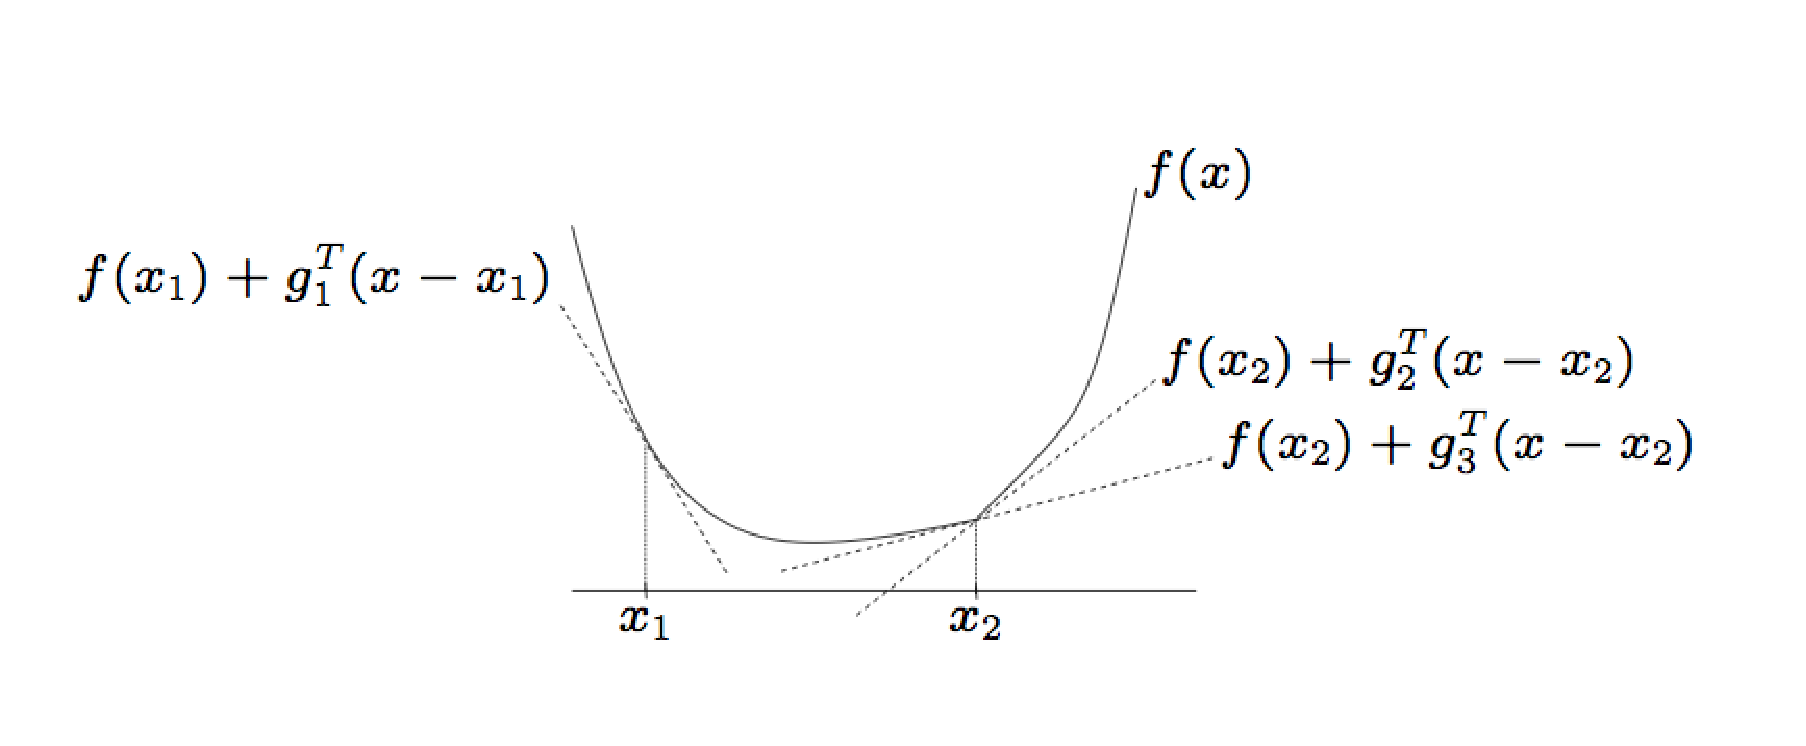
\includegraphics[width=0.8\textwidth]{subgrad_figure}
\end{center}


($g_1$ is a subgradient at $x_1$; $g_2$ and $g_3$ are subgradients at
$x_2$)%Probably unnecessary..



\medskip

\hrule\medskip
\Head{Computation of Subgradients}
\\
We apply a recursive procedure: For each atomic function, 
we implement a method that computes its subgradient. The subgradient of a
general expression can be computed using the composition rule:
\begin{itemize}

\item Let $f(x) = h(f_1(x), \ldots, f_k(x))$ with $h$ convex non-decreasing,
  $f_i$ convex.
\item Find $q \in \partial h(f_1(x), \ldots, f_k(x))$,  $g_i \in \partial
  f_i(x)$
\item Then $g = q_1 g_1 + q_2 g_2 + \cdots + q_k g_k  \in \partial f(x)$

\end{itemize}

\medskip

\hrule\medskip
\Head{Subgradient Methods}
\\
The subgradient method is similar to gradient descent methods for minimizing differentiable functions.

\begin{itemize}
\item At $x^{(k)}$, find $g^{(k)} \in f(x^{(k)})$.
\item Set the next point as $x^{(k+1)}:=x^{(k)}-\alpha_kg^{(k)}$, where $\alpha_k$ is $k$-th step size.

\end{itemize}

\medskip

\end{textblock}

\begin{textblock}{7.0}(8,1.5)

\hrule\medskip
\Head{Example Code}
\begin{verbatim}
from spy import *
x = var('x')
y = var('y')
ex = max(x+y,2*x-y) + abs(x)
constraints = [greater(y,0),less(x,y)]
prob = minimize(ex, constraints)
prob.solve()
\end{verbatim}

\medskip

\hrule\medskip
\Head{Expression Class}
\begin{itemize}
\item Currently, \verb'SPY' only supports scalar real variables and scalar-valued expressions.
\item Internally, an expression is stored as a tree.
\begin{center}
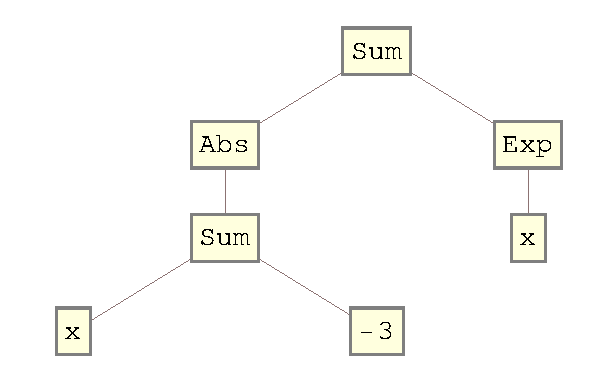
\includegraphics[width=0.6\textwidth]{poster/expr}
\end{center}
The tree above corresponds to the following mathematical expression:
\begin{equation*}
|x-3|+e^x \; .
\end{equation*}
\item Convexity or concavity of an expression is not tested at construction time.
\end{itemize}

\bigskip

\hrule\medskip
\Head{Constraint Class}
\\
 A constraint is an inequality of the form 
$(\mbox{convex}) \le (\text{concave})$ or an equality of the form
$(\text{affine}) = (\text{affine})$.

\bigskip

\hrule\medskip
\Head{Problem Class}
\\
A problem is a triplet of the form (minimize/maximize, objective, list of
constraints). The problem class contains a \verb'solve' method which
solves the specified problem using subgradient methods.


\medskip


\end{textblock}

\begin{textblock}{7.0}(16,1.5)

\hrule\medskip
\Head{Using SPY}
\begin{itemize}
\item Declaring variables: \\
One can declare a variable using the following syntax.
\begin{verbatim}
x = var('x')
\end{verbatim}
The object \verb'x' is a symbolic link to the variable with the identifier string \verb,'x',.
\item Forming expressions: \\
The following line creates an expression named \verb'ex'.
\begin{verbatim}
ex = abs(x - 3) + exp(x)
\end{verbatim}
\verb'SPY' does not attempt to simplify a given expression.
\item Computing values and subgradients of expressions: \\
The following code computes the value and a subgradient at a point given by \verb'varmap'.
\begin{verbatim}
varmap = {'x': 1.5, 'y': -2}
val    = ex.get_value(varmap)
g      = ex.subgrad(varmap)
\end{verbatim}
To represent a point, users should use a dictionary rather than a list of values.
\item Specifying constraints: \\
One can use \verb'leq', \verb'eq', or \verb'geq' to construct a constraint object.
\begin{verbatim}
cons = leq(norm2([x1, x2]), y)
\end{verbatim}
At construction time, \verb'SPY' will automatically check if inequalities and equalities follow the DCP ruleset.
\item Solving an optimization problem:
\begin{verbatim}
myprob = minimize(ex, [cons1, cons2])
(optval, optpoint) = myprob.solve()
\end{verbatim}
The lines above minimizes \verb'ex' subject to two constraints \verb'cons1' and \verb'cons2' using the subgradient method. As a result, the optimal point as well as the objective value at that point will be returned. Advanced users can specify the step size rule used by the method.
\item Available library functions:
\begin{itemize}
\item \verb'abs', \verb'max', \verb'min', \verb'pos'
\item \verb'exp', \verb'log', \verb'log_sum_exp', \verb'rel_entr'
\item \verb'norm1', \verb'norm2', \verb'berhu', \verb'huber'
\item \verb'power', \verb'power_pos', \verb'square', \verb'square_pos', \\ \verb'sqrt', \verb'geo_mean', \verb'quad_over_lin'
\end{itemize}
\end{itemize}

\medskip

\hrule\medskip
\Head{Limitations and Extension Ideas}
\begin{itemize}
\item Support vectors and matrices.
\item Have more library functions.
\item Support more complicated 
\end{itemize}

\medskip

\end{textblock}

\end{document}
